\documentclass[aspectratio=149] {beamer}
\usecolortheme{crane}
\usepackage[crane]{katescodingstyles}
\usepackage{hyperref}


\setbeamertemplate{footline}[frame number alone]


\hypersetup{
	colorlinks=true,
	urlcolor=accentshade
	}
\urlstyle{same}

\newcommand{\pyTWO}[1][]{
  \begin{tikzpicture}[remember picture,overlay,#1]
    \node {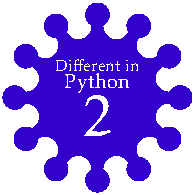
\includegraphics[scale=.5]{pyTWO}};
  \end{tikzpicture}% 
}




\title[OOP!]{Object-Oriented Python!}
\subtitle{classes, subclasses, self and super}
\author{Kate MacInnis}
\institute{PyLadies-ATX Tech Talk\\June 4, 2015}
\date{}




\begin{document}

\begin{frame}
\titlepage
\end{frame}


\begin{frame}[fragile]{In this presentation\dots}
  All code samples are written with Python 3 in mind.
  
  \bigskip
  
  
  We will be editing code in a text editor, and running it in the interactive console. When we make changes to our text file, we will need to do the following:
  
  ~\hfill
  \begin{columns}
    \begin{column}[t]{.4\textwidth}
      {\small if using the built-in console:}
      \begin{codeblock}
        quit()
        python3
        from example import *
      \end{codeblock}
    \end{column}
   
    \begin{column}[t]{.4\textwidth}
      {\small if using ipython:}
      \begin{codeblock}
        run example.py
      \end{codeblock}
    \end{column}
  \end{columns}
  
  \bigskip
  
  
  You will need to do this after each change to the code in a text file.
  
  
\end{frame}



\begin{frame}[fragile]{Before we begin\dots some nifty python tricks}

  Save this in a text file called stars.py:
  
  \begin{smallpythoncode}
    def func0(myvar):
        print('myvar = {}'.format(myvar))
        print('type(myvar) = {}'.format(type(myvar)))
    
    def func1(*args):
        print('args = {}'.format(args))
        print('type(args) = {}'.format(type(args)))
    
    def func2(myvar, *args):
        print('myvar = {}'.format(myvar))
        print('args = {}'.format(args))
    
    def func3(myvar, *args, **kwargs):
        print('myvar = {}'.format(myvar))
        print('args = {}'.format(args))
        print('kwargs = {}'.format(kwargs))
        print('type(kwargs) = {}'.format(type(kwargs)))
  \end{smallpythoncode}


\end{frame}






\begin{frame}[fragile,t]{ Nifty python tricks}

  \begin{columns}
    \begin{column}[t]{.48\textwidth}
      stars.py (for reference)
      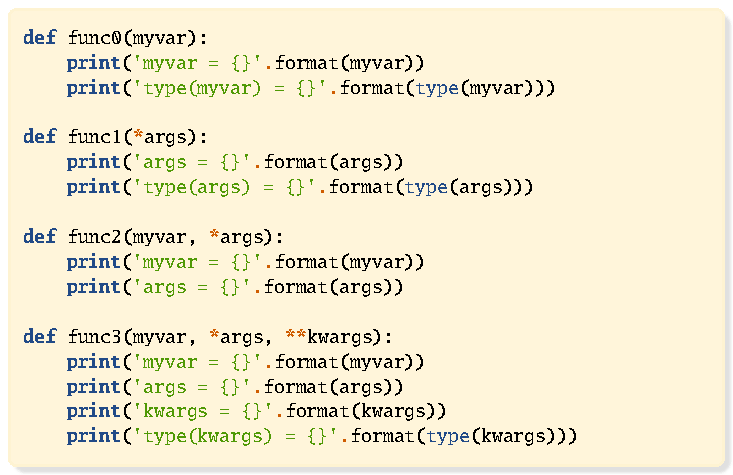
\includegraphics[scale=.85, trim= 0 0 7cm 0, clip]{stars.pdf}
    \end{column}
   
    \begin{column}[t]{.48\textwidth}
      Predict the outcome of each of these, 
      and test them in the console:
      \begin{pythoncode}
        func0(5)
        func0()
        func0(1,2,3)	
      \end{pythoncode}
  
      \pause
      \begin{pythoncode}
        func1(5)
        func1()
        func1(1,2,3)	
      \end{pythoncode}
    \end{column}
  \end{columns}

\end{frame}


\begin{frame}[fragile,t]{ Nifty python tricks}

  \begin{columns}
    \begin{column}[t]{.48\textwidth}
      stars.py (for reference)
      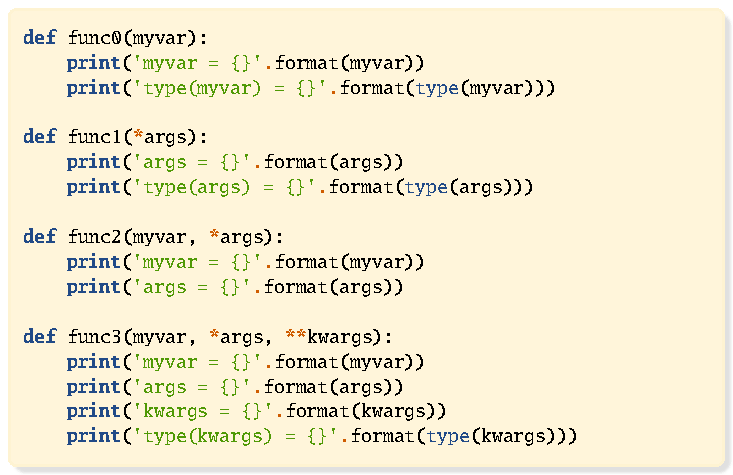
\includegraphics[scale=.85, trim= 0 0 7cm 0, clip]{stars.pdf}
    \end{column}
   
    \begin{column}[t]{.48\textwidth}
      And these:
      \begin{pythoncode}
        func2(1,2,3,4,5)
        func2()
        func2(1)
        func2(colors)
      \end{pythoncode}
  
      \pause
      \begin{pythoncode}
        func2(*colors)
        func2(*triples)
        func2(*range(8))
      \end{pythoncode}
    \end{column}
  \end{columns}

\end{frame}


\begin{frame}[fragile,t]{ Nifty python tricks}

  \begin{columns}
    \begin{column}[t]{.48\textwidth}
      stars.py (for reference)
      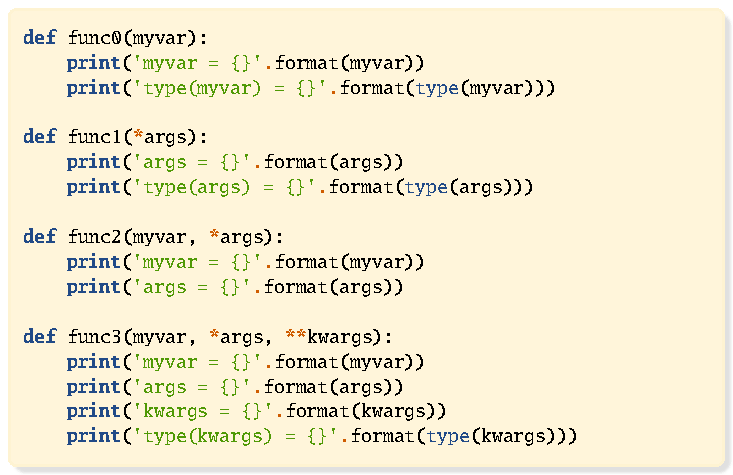
\includegraphics[scale=.85, trim= 0 0 7cm 0, clip]{stars.pdf}
    \end{column}
   
    \begin{column}[t]{.48\textwidth}
      And these:
      \begin{pythoncode}
        func3(1,2,3,4,5)
        func3(1,2,3,a=88,b=99)        
        func3(a=55,b=66,myvar=0)
        func3(mathyfolks)
        func3(0, mathyfolks)
      \end{pythoncode}
  
      \pause
      \begin{pythoncode}
        func3(0,**mathyfolks)
        func3(*colors,**mathyfolks)
        func3(**mathyfolks)
        func3(**junk)
      \end{pythoncode}
    \end{column}
  \end{columns}

\end{frame}


\begin{frame}[fragile]{Nifty python tricks}

  \textbf{\Large Star Operators} 
  \begin{itemize}
    \onslide<2->{\item Within the parameters of a function definition:} 
      \begin{itemize}
        \onslide<3->{\item \inlinett{*} packs all the extra positional arguments into a tuple} 
        \onslide<5->{\item \inlinett{**} packs all the extra keyword arguments into a dictionary }
      \end{itemize}
    \onslide<2->{\item Within the arguments of a function call:}  
      \begin{itemize}
        \onslide<4->{\item \inlinett{*} unpacks a tuple, list, or other sequence type into positional arguments} 
        \onslide<6->{\item \inlinett{**} unpacks a dictionary into keyword arguments }
      \end{itemize}
  \end{itemize}

\end{frame}


\begin{frame}[fragile]{Nifty python tricks}

  A \keyword{decorator} is a special kind of function, 
  one that accepts a function as input, 
  and returns a replacement function\textsuperscript{*}.

  \note{*It doesn't actually have to be a function, it just has to be callable.}

  \medskip \pause

  \begin{columns}

    \begin{column}[b]{.65\textwidth}

      \begin{smallpythoncode}
      def my_decorator(original_function):
    
          def replacement_function():
              print('Do stuff before')
              original_function()
              print('Do stuff after')

          return replacement_function

      def hello_world():
          print('Hello world!')

      f = my_decorator(hello_world)

      \end{smallpythoncode}
      
    \end{column}
    \begin{column}[b]{.3\textwidth}

      What will happen\\when you call \inline`f()`?

      \vspace{1cm}

    \end{column}
  \end{columns}
\end{frame}


\begin{frame}[fragile]{Nifty python tricks}

  A common pattern emerged that people would redefine the function variable to mean the function with the decorator applied.
  \begin{pythoncode}
    hello_word = my_decorator(hello_world)
  \end{pythoncode}
  
  \pause \medskip
  
  Beginning in Python 2.4, if you want to {always} use a decorator when you call a function, you can use use this syntax 
  at the function's definition:
  \begin{pythoncode}
    @my_decorator
    def hello_world():
        print('Hello world!')
  \end{pythoncode}

\end{frame}

\begin{frame}[fragile]{Nifty python tricks}

  {\large Some Uses For Decorators}


  \begin{itemize}
    \item Caching the results of time-consuming calculations
    \item Requiring that users are logged in before running the function
    \item Checking that users have permission to run that function
    \item To log the time it takes for the function to run
  \end{itemize}

  If you're interested in seeing the code for some decorators,
  see: \url{https://wiki.python.org/moin/PythonDecoratorLibrary}

\end{frame}





{
\setbeamercolor{background canvas}{bg=craneorange!90}
\begin{frame}{And now\dots}
  \vspace{-5ex} \pause
  \begin{center}  
    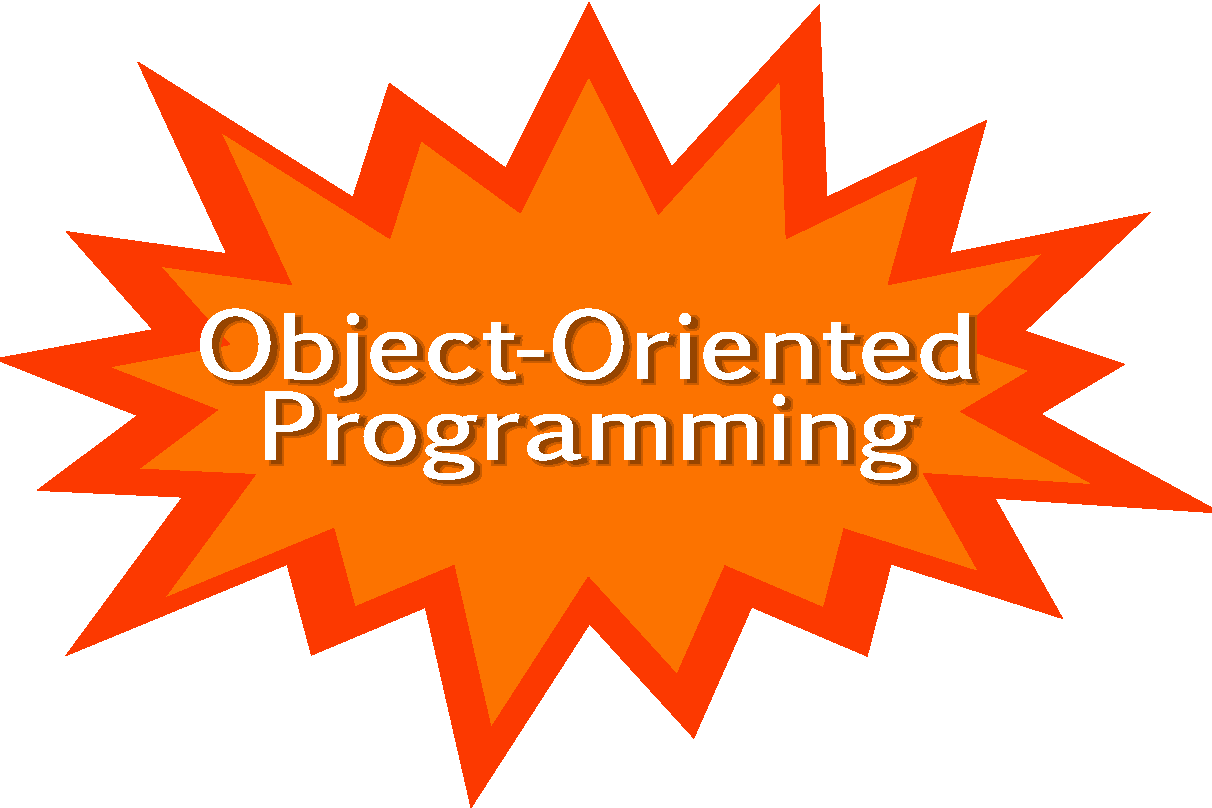
\includegraphics[scale=.6]{starburstsf}
  \end{center}
\end{frame}
}





\begin{frame}[fragile]{A quick note\dots}

  For this presentation, we won't always begin with the ``right'' way to do things.

  \medskip

  I will frequently start with a not-great approach, just so we can examine the problems.
  We will refactor the code and make it better.
  
  \medskip \pause
  
  I will also ask from time to time what you expect to happen in a situation.
  ``Wrong'' answers will be embraced enthusiastically.  
  Some of the ideas that I will introduce are a little bit counter-intuitive.
  To really understand, we will need to examine our intuition,
  see how it is different from reality, 
  and take a look at the reason for those differences. 

\end{frame}





\begin{frame}[fragile]{Programming Paradigms}

  In \keyword{Procedural Programming},
  the focus is on step-by-step instructions for the computer.
  These procedures will operate on data, but the procedures 
  and the data structures are sort of separate concepts.

  \bigskip \pause

  In \keyword{Object-Oriented Programming},
  the code is conceptualized around objects 
  that bundle together relevant values (attributes) and functions (methods).

  \bigskip \pause

  There are other paradigms, but these are the two that Python is most commonly used for.

\end{frame}

\begin{frame}[fragile]{What kinds of objects can you make?}

  \begin{itemize}
  \item Bank Account
  	\begin{itemize}
  		\item attributes: balance, minimum balance, interest rate
  		\item methods: deposit, withdraw, check balance
  	\end{itemize}
  \item GUI Widget
  	\begin{itemize}
  		\item attributes:  location, size, color
  		\item methods: click, drag, mouseover
  	\end{itemize}
  \item Game Character
  	\begin{itemize}
  		\item attributes:  strength, experience points, inventory
  		\item methods:  move, interact, attack
  	\end{itemize}
  \item User
  	\begin{itemize}
  		\item attributes:  name, password, other profile information
  		\item methods: log in, edit profile, 
  	\end{itemize}
  \end{itemize}


\end{frame}


\begin{frame}[fragile]{Our first homemade object}
  \small
  Let's create our first class:

  \begin{pythoncode}
    class Thing:
        pass
  \end{pythoncode}    

  That's all it takes!

  \pause \medskip

  Now that we have a new class, we can create an \keyword{instance} of that class: 
  \begin{pythoncode}
    thing = Thing()
  \end{pythoncode}

  \pause

  And we can assign attributes to this object:
  \begin{pythoncode}
    thing.a = 5
    thing.b = 'hi there'
  \end{pythoncode}

  \pause
  ~\hfill Of course, it doesn't actually do anything\dots

\end{frame}

\begin{frame}[fragile]{Our first interesting object}

  Most interesting objects need to be \keyword{initialized}.

  \pause \medskip

  In python, we define an \inline`__init__` 
  method on our class to handle the initialization.

  \pause \medskip

  \begin{pythoncode}
  class Rectangle:
      def __init__(self, width, length):
          self.width = width
          self.length = length
        
  \end{pythoncode}

  (Note that there are double underscores at the start and end of the word init.)

  \medskip

  The \inline`__init__` method that we are defining here is sometimes called a magic method.  You can call it directly, but python uses this method automatically whenever a new instance of the class is created.
\end{frame}


\begin{frame}[fragile]{Important Points on \_\_init\_\_}

  \begin{itemize}

    \item The first argument passed to init is the newly created instance of the class. Call this \inline`self`.  

    (This is not specific to init: the first argument passed to any method is the instance, and it should always be called self. Python wont enforce this, but your fellow coders and future self will thank you.)

    \bigskip

    \item Notice that \inline`__init__` does not return anything!  It sets the values of attributes on the newly created object.  It should never contain a return statement
  \end{itemize}

\end{frame}


\begin{frame}[fragile,t]{Our first interesting object}


  \begin{columns}
    \begin{column}[t]{.59\textwidth}
      To make this example more useful,\\lets add another method. 
 
      %\vspace{-5ex}
      \only<1|handout:0>{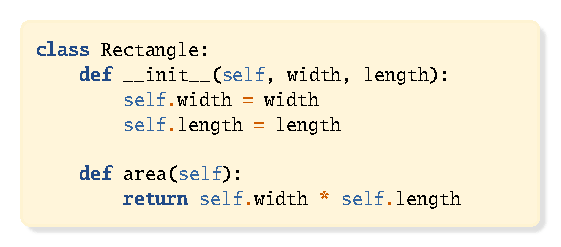
\includegraphics{rectangle1}}
      \pause
      \begin{smallpythoncode}
        class Rectangle:
            def __init__(self, width, length):
                self.width = width
                self.length = length
    
            def area(self):
                return self.width * self.length
      \end{smallpythoncode}
    \end{column}
    \begin{column}[t]{.42\textwidth}
      Let's make a rectangle!  

      In the console:
      \begin{pythoncode}
        r = Rectangle(3,5)
        r.width
        r.length
        r.area
        r.area()
        dir(r)
        isinstance(r,Rectangle)
        r
      \end{pythoncode}
    \end{column}
  \end{columns}

  \bigskip \pause
  
  We will want a better representation of our rectangle than \inline`<__main__.Rectangle at 0x101e45ba8>`

\end{frame}


\begin{frame}[fragile]{Better represenation}

  There are two special methods that we can use to return a string representation of our objects: \inline`__str__` and \inline`__repr__`. \pause

  \begin{itemize}

    \item \inline`__str__` should be used for a string representation that is useful to 
    the end-user. \pause

    \item \inline`__repr__` should be used for a string representation that is useful to 
    the programmer.  This is what the console shows.

    \medskip

    It is considered a good practice to make the output of \inline`__repr__` something that can recreate the object, if possible.
     If this is not possible, a useful description for debugging purposes should be enclosed in \inline`< >`.

    \medskip

    If a class has no \inline`__str__` method, but has \inline`__repr__`, \inline`__repr__` will be used whenever \inline`__str__` is called for.

  \end{itemize}

\end{frame}

\begin{frame}[fragile]{Better representation}

Let's add a \inline`__repr__` method to our class:
\small
\begin{pythoncode}
class Rectangle:
    def __init__(self, width, length):
        self.width = width
        self.length = length

    def __repr__(self):
        return 'Rectangle(%s,%s)' % (self.width, self.length)
    
    def area(self):
        return self.width * self.length

\end{pythoncode}

\medskip 

Load the new code in the interactive interpreter, 
make a new rectangle object, and see how it is displayed.


\end{frame}


\begin{frame}[fragile]{One more method\dots maybe an attribute?}
  
  Suppose we need the length of the diagonal of our rectangle.
  
  \pause \smallskip
  
  Since the diagonal of a rectangle with sides $l$ and $w$ 
  is $\sqrt{l^2 + w^2}$,\\[-1pt]
  we can write a method:
  
  \smallskip \pause
   
  \only<3|handout:0>{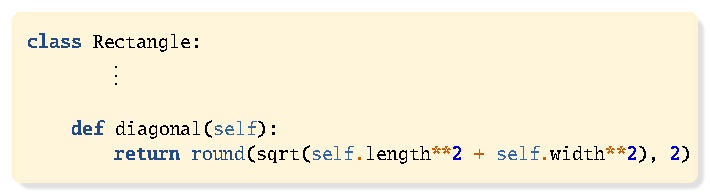
\includegraphics[page=1]{diagonal}}
  \onslide<4->
  \includegraphics[page=2]{diagonal}
  
  The \inline`@property` decorator makes a method seem like an
  attribute.
  
  
\end{frame}




\begin{frame}[fragile]{Subclassing}

  We can create a subclass of any existing class---whether that class is a built-in class or something that we've made ourselves.

  \medskip \pause

  In shapes.py, add:
  \begin{pythoncode}
    class Square(Rectangle):
        def __init__(self, side):
            self.side = side
  \end{pythoncode}

  \medskip \pause

  In the console:
  \begin{pythoncode}
    s = Square(5)
    dir(s)
  \end{pythoncode}

  \pause

  Where does the \inline`area` method come from? \\
  What happens when you run \inline`s.area()`?

\end{frame}

\begin{frame}[fragile]{Subclassing}

  When subclassing, you must make sure that all necessary attributes for the superclass are initialized on your subclass.

  \medskip

  We could do that manually, or we could use the \inline`super` function\textsuperscript{*}. 

  \medskip

  The \inline`super` function returns the superclass of the class you're currently writing.

\end{frame}

\begin{frame}[fragile]{Subclassing}

  We can fix our \inline`Square` class like this:

  \begin{pythoncode}
    class Square(Rectangle):
        def __init__(self, side):
            self.side = side
            super().__init__(side, side)
  \end{pythoncode} 
  
  \pause
  
  \pyTWO[xshift=12cm,yshift=1cm] \pause

  Now, try this in the terminal:

    \begin{columns}
      \begin{column}[b]{.48\textwidth}
          \begin{pythoncode}
            s = Square(8)
            s.side
            s.width
            s.height
            s.area()
      
          \end{pythoncode}
      \end{column}
      \begin{column}[b]{.48\textwidth}
        \begin{pythoncode}
          isinstance(s, Square)
          isinstance(s, Rectangle)
          s
        \end{pythoncode}

      \end{column}
    \end{columns}  

\end{frame}


\begin{frame}[fragile]{Refactoring time}
  
  When you find yourself having to make lots and lots of little changes
  every time you make a new subclass, it's time to take a step back,
  think over your entire project, and refactor your code.
  
  \bigskip
  
  Let's create a new base class, \inline`Shape`, which we won't instantiate directly,
  but will hold the some code that will be common to all our shapes.
  
\end{frame}



\begin{frame}[fragile]{Refactoring time}

\small
\begin{pythoncode}
  class Shape:
      def __init__(self, *args, **kwargs): 
          self.args = args
          self.kwargs = kwargs |\pause|

      def __repr__(self): |\pause|
          shape = self.__class__.__name__ |\pause|
          all_args = []
          for arg in self.args:
              all_args.append(repr(arg))  |\pause|
          for kw, arg in self.kwargs.items():
              all_args.append('{0}={1}'.format(kw, repr(arg)))  |\pause|
          comma_sep_args = ', '.join(all_args) |\pause|
          return '{0}({1})'.format(shape, comma_sep_args)
\end{pythoncode}


\end{frame}


\begin{frame}[fragile]{Changes to the Base Class}

  Let's assume that we want every subclass of shape to be able to calculate its area.

  \pause

  \begin{pythoncode}
    class Shape:
            |$\vdots$|
        def area(self):
            raise NotImplementedError
        
  \end{pythoncode}
  
  \medskip \pause
  
  This doesn't force subclasses to implement an area method, 
  it's just a convention for working with other programmers.
  
  \smallskip \pause
  
  If you need to absolutely force certain methods to be implemented, 
  look into the  \inline`abc` module of the standard library.
  That will allow you to create an \keyword{Abstract Base Class} 
  to which you can add abstract methods which must be implemented on 
  any subclass before the subclass can be instantiated. 


\end{frame}


\begin{frame}[fragile]{Changes to the Base Class}

Finally, let's make \inline`shape` a property of our base class:


  \begin{pythoncode}
    class Shape:
            |$\vdots$|
        @property
        def shape(self):
            return self.__class__.__name__

  \end{pythoncode}



\end{frame}


\begin{frame}[fragile]{Now let's get subclassin'}

There are two main ways that we could handle the parameters for initializing the Rectangle class:
\begin{pythoncode}
class Rectangle(Shape):
    def __init__(self, width, length):
        self.width = width
        self.length = length
        super().__init__(width, length)
\end{pythoncode}

\begin{pythoncode}
class Rectangle(Shape):
    def __init__(self, *args):
        self.width, self.length = sorted(args)
        super().__init__(*args)
\end{pythoncode}

\end{frame}


\begin{frame}[fragile]{Putting conditions on init}

  \begin{pythoncode}
    class Triangle(Shape):
    
        def __init__(self, *args):
            a, b, c = sorted(args)
            if a + b <= c:
                raise ValueError('Cannot construct triangle with sides given.')
            self.sides = (a,b,c)
            super().__init__(*args)
    
        def area(self):
            semi = sum(self.sides)/2
            a,b,c = self.sides
            return math.sqrt(semi*(semi-a)*(semi-b)*(semi-c))
    
  \end{pythoncode}

\end{frame}



\begin{frame}[fragile]{Errors are objects too}

  You can subclass errors, to get your own, special ones: \pause
  \begin{pythoncode}
    class GeometryError(ValueError):
        pass
  \end{pythoncode}
  
  \medskip \pause
  
  Let's change the previous error line to use our new error:
  
  \begin{smallpythoncode}
    raise GeometryError('Cannot construct triangle with sides given.')
  \end{smallpythoncode}
  



\end{frame}

\begin{frame}[fragile]{Your turn\dots}

  Make a \inline`Circle` class.
  
  \medskip\pause
  
  This is one possible solution:
      \begin{pythoncode}
        class Circle(Shape):
  
            def __init__(self, radius):
                self.radius = radius
                super().__init__(radius)
    
            def area(self):
                return 3.14 * self.radius**2
      \end{pythoncode}


\end{frame}


\begin{frame}[fragile]{Equality!}

  Load shapes.py into the console, and try this:
  
  \begin{pythoncode}
    Circle(3) == Circle(3)
  \end{pythoncode}
  \pause
  What happens? Why?
  
  \medskip\pause
  
  If python doesn't have any instructions on how to determine equality,
  it goes by an object's location in memory.  
  
  \medskip
  
  Since these are two different instances, python says they're not equal,
  even though they're identical.
  
  \medskip
  
  If we want different behavior, we have to tell it how to determine equality.


\end{frame}


\begin{frame}[fragile]{Equality!}

  To tell python how to determine equality, we add another special method,
  called \inline`__eq__`: \pause

  \begin{pythoncode}
    class Shape:
         |\vdots|
        def __eq__(self, other):
            if self.__class__ != other.__class__:
                return False
            if (self.args == other.args):
                return True
            return False
  \end{pythoncode}

  \medskip \pause
  
  Now try \inline`Circle(3) == Circle(3)` again.


\end{frame}


\begin{frame}[fragile]{Operator Overloading / More Special Methods}
  
  Open \inline`fractions.py` in a text editor.
  \tiny
  \begin{pythoncode}
    class Fraction:
        def __init__(self, numerator, denominator=1):
            if not all([isinstance(i,int) for i in (numerator,denominator)]):
                raise ValueError('Arguments of Fraction must be integers')
            g = gcd(numerator,denominator)
            self.n = int(numerator/g)
            self.d = int(denominator/g)

        def __neg__(self):
            return Fraction(-self.n,self.d)

        def __abs__(self):
            return Fraction(abs(self.n),abs(self.d))

        def __add__(self, other):
            if not isinstance(other, Fraction):
                other = Fraction(other)
            n = self.n * other.d + self.d * other.n
            d = self.d * other.d
            return Fraction(n, d)

        def __sub__(self, other):
            return self + (-other)

        def __mul__(self, other):
            if not isinstance(other, Fraction):
                other = Fraction(other)
            n1, d1 = self.n, self.d
            n2, d2 = other.n, other.d
            return Fraction(n1*n2, d1*d2)

        def __truediv__(self, other):
            if not isinstance(other, Fraction):
                other = Fraction(other)
            n1, d1 = self.n, self.d
            n2, d2 = other.n, other.d
            return Fraction(n1*d2, d1*n2)

        def __eq__(self, other):
            return (self.n, self.d) == (other.n, other.d)        

        def __str__(self):
            return "%s/%s" % (self.n, self.d)

        def __repr__(self):
            return 'Fraction(%s,%s)' % (self.n, self.d)
  \end{pythoncode}
\end{frame}


\begin{frame}[fragile]{Operator Overloading / More Special Methods}
  Here are some common operators and the methods to implement on your classes. 
\note{   \inline`obj` is the instance of the object that you are writing a class for}

  \small \vspace{-4ex}
  
  
    \begin{columns}
      \begin{column}{.48\textwidth}
        \begin{center}
          \begin{tabular}{ccl}
            \hline
            operation & method\\
            \hline
               \inline`obj + other` & \inline`__add__` \\
               \inline`obj - other` & \inline`__sub__` \\
               \inline`obj * other` & \inline`__mul__` \\
               \inline`obj // other` & \inline`__floordiv__` \\
               \inline`obj / other` * & \inline`__div__` \\
               \inline`obj / other` ** & \inline`__truediv__` \\
               \inline`obj % other` & \inline`__mod__` \\
               \inline`obj ** other` & \inline`__pow__` \\
            \hline
          \end{tabular}
        \end{center}        
      \end{column}
      \begin{column}{.48\textwidth}
        \begin{center}
          \begin{tabular}{ccl}
            \hline
            operation & method\\
            \hline
            \inline`other + obj` & \inline`__radd__` \\
            \inline`other - obj` & \inline`__rsub__` \\
            \inline`other * obj` & \inline`__rmul__` \\
            \inline`other // obj` & \inline`__rfloordiv__` \\
            \inline`other / obj` * & \inline`__rdiv__` \\
            \inline`other / obj` ** & \inline`__rtruediv__` \\
            \inline`other % obj` & \inline`__rmod__` \\
            \inline`other ** obj` & \inline`__rpow__` \\
            \hline
          \end{tabular}
        \end{center}
      \end{column}
    \end{columns}  


\bigskip
\scriptsize * only in Python 2\\
 ** in Python 3, or in Python 2, with \inlinett{\tiny from \_\_future\_\_ import division} 
  
  
\end{frame}


\begin{frame}[fragile]{Operator Overloading / More Special Methods}
  
  We implemented \inline`__eq__` on our shapes class, but there are more comparison operators than just that.
  
  \small
          \begin{center}
          \begin{tabular}{cc}
            \hline
            operation & method\\
            \hline
            \inline`obj == other` & \inline`__eq__` \\
            \inline`obj != other` & \inline`__ne__` \\
            \inline`obj < other` & \inline`__lt__` \\
            \inline`obj > other` & \inline`__gt__` \\
            \inline`obj <= other` & \inline`__le__` \\
            \inline`obj >= other` & \inline`__ge__` \\
            \hline
          \end{tabular}
        \end{center}
        \normalsize
        For our fractions class,
        we could either implement all six comparisons,
        or we could implement \inline`__eq__` plus just one
        of \inline`__lt__`, \inline`__gt__`, \inline`__le__`,
        or \inline`__ge__` and use the 
        class decorator
        \inline`@total_ordering`.
  
\end{frame}



\begin{frame}[fragile]{Pythonic Protocols}
  
  Python doesn't have interfaces the way Java and many other staticly-typed languages do.
  \note{You *can* create interfaces in Python (see Zope) but it's not necessary the way it is in other languages,
  because Python generally relies on Duck-Typing and supports multiple inheritance}
  
  \bigskip
  
  Because traditionally Python relies heavily on \keyword{duck typing}, for your object to be treated
  like one of a category of objects, all you have to is implement the right methods.  
  This is sometimes loosely called a Protocol.
  

  
\end{frame}




\begin{frame}[fragile]{Protocols}
  
  To create a container object, implement:
  \begin{itemize}
  	\item \inline`__len__`
    \item \inline`__getitem__` \pause
    \item \inline`__setitem__` (if you want a mutable container)
    \item \inline`__delitem__` (if you want a mutable container) \pause
    \item \inline`__iter__` (if you want your container to be iterable)
  \end{itemize}

  \medskip \pause
  
  To create an iterator, either write a generator (a function that uses the \inline`yield` statement to return a sequence of values) or write a new class that implements:
  \begin{itemize}
    \item \inline`__iter__`
    \item \inline`__next__` \pyTWO[xshift=3cm]
  \end{itemize}

  
\end{frame}


\begin{frame}[fragile]{Protocols}
  \setlength{\unitlength}{1cm}
  \begin{picture}(6,.01)
    \put(4,-3.3){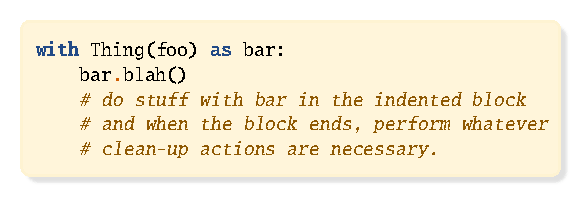
\includegraphics[scale=.85]{with}}
  \end{picture}
  
  To create a context manager object that works in a \inline`with` statement:
    
  \begin{itemize}
    \item \inline`__enter__`
    \item \inline`__exit__`
  \end{itemize}
  
  \vspace{1.2cm}
  
  \medskip \pause  
  
  To create an object that can be called like a function, implement:
  \begin{itemize}
    \item \inline`__call__`
  \end{itemize}
  

  
\end{frame}

\begin{frame}[fragile]{Subclassing Built-In Types}
  
  
  Although duck typing is the ``Pythonic'' way, if your object needs to interact with code that will do \inline`isinstance` checks,
  you should subclass the type that you need it to be.  
  You can then change the methods however you want.
  \note{Remember, when you write a method on a subclass, the method with the same name on the superclass is replaced.}
  
  
\end{frame}

\begin{frame}[fragile]{Multiple Inheritance}
  
  Python allows a class to inherit from multiple classes.
  
  
\end{frame}



\tikzset{
    invisible/.style={opacity=0},
    visible on/.style={alt={#1{}{invisible}}},
    alt/.code args={<#1>#2#3}{%
      \alt<#1>{\pgfkeysalso{#2}}{\pgfkeysalso{#3}} % \pgfkeysalso doesn't change the path
    },
  }

\begin{frame}[fragile]{Multiple Inheritance: Method Resolution Order}
  In uncomplicated cases, when Python is looking for a method or attribute, 
  it checks the parent classes from left to right, depth first. \pause
    \begin{columns}
      \begin{column}{.3\textwidth}
        \scriptsize 
        \begin{pythoncode}
          class X:
              pass

          class Y(X):
              pass

          class W:
              pass

          class Z(W):
              pass

          class J:
              pass

          class Alpha(Y,J,Z):
              pass
        \end{pythoncode}
        \pause
      \end{column}
      \begin{column}{.71\textwidth}
          \begin{center}
            \begin{tikzpicture}[node distance=1.8cm,
              font=\Large\rmfamily,
              class/.style = {
                shape=rectangle, 
                rounded corners,
                draw, align=center,
                top color=craneorange!10, 
                bottom color=accentshade!20
                }
                ]
                \begin{scope}
                  \node[class] (Alpha) {Alpha};
                  \node[class] (Y) [above left of=Alpha] {Y}; 
                  \node[class] (X) [above of=Y] {X};
                  \node[class] (J) [above of=Alpha] {J};
                  \node[class] (Z) [above right of=Alpha] {Z};
                  \node[class] (W) [above of=Z] {W};
                  \path (Alpha) edge (Y) edge(J) edge (Z);
                  \path (Y) edge (X);
                  \path (Z) edge (W);
                \end{scope}
                \begin{scope}[red, very thick, ->]
                  \draw [visible on=<4->] (Alpha) -- (Y);
                  \draw [visible on=<5->] (Y) -- (X);
                  \draw [visible on=<6->] (X) -- (J);
                  \draw [visible on=<7->] (J) -- (Z);
                  \draw [visible on=<8->] (Z) -- (W);
                \end{scope}
            \end{tikzpicture}
            \scriptsize
            \onslide<9->
            \begin{codeblock}
              >>> Alpha.mro()
              [<class 'multi.Alpha'>, <class 'multi.Y'>, 
              <class 'multi.X'>, <class 'multi.J'>, 
              <class 'multi.Z'>, <class 'multi.W'>, <class 'object'>]
            \end{codeblock}
          \end{center}
      \end{column}
    \end{columns}    
\end{frame}


\begin{frame}[fragile]{Multiple Inheritance: Method Resolution Order}
  
  {MROs get more complicated if the diagram of classes contains cycles.}
  
  \onslide<2->
  \begin{columns}
      \begin{column}{.27\textwidth}
        \begin{pythoncode}  
          class A:
              #stuff

          class B(A):
              #stuff

          class C(A):
              #stuff

          class D(B,C):
              #stuff
        \end{pythoncode}

      \end{column}
      \begin{column}{.73\textwidth}
        \begin{center}
          \begin{tikzpicture}[node distance=2cm,
            font=\Large\rmfamily,
            class/.style = {
              shape=rectangle, 
              rounded corners,
              draw, align=center,
              top color=craneorange!10, 
              bottom color=accentshade!20
              }
              ]
            \begin{scope} 
              \node[class] (D)                    {D};
              \node[class] (B) [above left of=D]  {B};
              \node[class] (A) [above right of=B] {A};
              \node[class] (C) [above right of=D] {C};

              \path (D) edge (B) edge (C);
              \path (A) edge (B) edge (C);  
            \end{scope}
            \begin{scope}[very thick, red, ->]
              \draw [visible on=<4->] (D) -> (B);
              \draw [visible on=<5->] (B) -> (C);
              \draw [visible on=<6->] (C) -> (A);
            \end{scope}
          \end{tikzpicture}
          
          \small
          \onslide<3->
          \begin{codeblock}
            >>> D.mro()
            [<class 'multi.D'>, <class 'multi.B'>, 
            <class 'multi.C'>, <class 'multi.A'>, 
            <class 'object'>]
          \end{codeblock}
          \note{Emphasize that it's important that if This is a parent class of That, then This must come after That in the MRO.}
        \end{center}
      \end{column}
    \end{columns}  
\end{frame}


\begin{frame}{Multiple Inheritance: Method Resolution Order}
  Now let's look at what happens when we actually call some methods from 
  a class that uses multiple inheritance.
\end{frame}

\begin{frame}[fragile]{Multiple Inheritance: Method Resolution Order}
    
  \begin{columns}
      \begin{column}{.38\textwidth}
        \scriptsize
        \vspace{-1em}
        \begin{pythoncode} 
          class A:
              def foo(self):
                  print('foo from A')

          class B(A):
              def foo(self):
                  print('foo from B')
                  super().foo()
              def bar(self):
                  print('bar from B')

          class C(A): |\LARGE|
              def foo(self):
                  print('foo from C')
                  super().foo()
              def bar(self):
                  print('bar from C')

          class D(B,C):
              def foo(self):
                  print('foo from D')
                  super().foo()
        \end{pythoncode}

      \end{column}
      \begin{column}{.58\textwidth}
        \begin{center}
          \begin{tikzpicture}[node distance=2cm,
            font=\Large\rmfamily,
            class/.style = {
              shape=rectangle, 
              rounded corners,
              draw, align=center,
              top color=craneorange!10, 
              bottom color=accentshade!20
              }
              ]
            \begin{scope} 
              \node[class] (D)                    {D};
              \node[class] (B) [above left of=D]  {B};
              \node[class] (A) [above right of=B] {A};
              \node[class] (C) [above right of=D] {C};

              \path (D) edge (B) edge (C);
              \path (A) edge (B) edge (C);  
            \end{scope}
            \begin{scope}[very thick, red, ->]
              \draw  (D) -> (B);
              \draw  (B) -> (C);
              \draw  (C) -> (A);
            \end{scope}
          \end{tikzpicture}
          \small
            \begin{columns}
              \begin{column}{.48\textwidth}
                \only<2|handout:0>{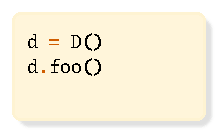
\includegraphics[page=1]{multdfoobar}} 
                \only<3->{\includegraphics[page=2]{multdfoobar}} 
              \end{column}
              \pause
              \begin{column}{.48\textwidth}
                \only<4|handout:0>{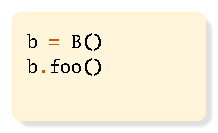
\includegraphics[page=1]{multbfoobar}} 
                \only<5>{\includegraphics[page=2]{multbfoobar}} 
              \end{column}
            \end{columns}  

        \end{center}
      \end{column}
    \end{columns}  
\end{frame}

\begin{frame}[fragile]{Multiple Inheritance: My Weirdest Example}
  
    \begin{columns}
      \begin{column}{.52\textwidth}
        \begin{pythoncode}
          class First:
              pass

          class Second(First):
              pass

          class Third(First, Second):
              pass
        \end{pythoncode}

      \end{column}
      \begin{column}{.48\textwidth}
        \begin{center}
          \begin{tikzpicture}[node distance=3.3cm,
            font=\LARGE\rmfamily,
            class/.style = {
              shape=rectangle, 
              rounded corners,
              draw, align=center,
              top color=craneorange!10, 
              bottom color=accentshade!20
              },
            ques/.style = {
              font=\huge\bfseries,
              color=red!80!blue,
            }
            ]
            \begin{scope}
              \node[class] (First) {First};
              \node[class] (Second) [below right of=First] {Second}; 
              \node[class] (Third) [below left of=Second] {Third}; 
              \path (First) edge (Second);
              \path (Second) edge (Third);
              \path (First) edge [bend right] (Third);
            \end{scope}
            \begin{scope}[very thick, red, ->]
              \draw [visible on=<2->] (Third) edge [bend left] node (Q1)[ques,left, visible on=<7->] {?} (First);
              \draw [visible on=<3->] (Third) -- node (Q3)[ques,below right=-1mm, visible on=<6->] {?} (Second);
              \draw [visible on=<4->] (Second) -- node(Q2)[ques, above right=-1mm, visible on=<5->] {?} (First);
              \node at (0.8,-2.2)[visible on=<8->,scale=5,ques] {???};
            \end{scope}

          \end{tikzpicture}
        \end{center}
      \end{column}
    \end{columns}  

  \onslide<9>
  Let's try running this code, and see what happens.
  
\end{frame}


\begin{frame}[fragile]{Multiple Inheritance: Important Points}
  \small
  Python's multiple inheritance allows you to create a class that inherits from more than one class.
  It's not as hard as some claim, but you do need to be aware of a few things:
  
  \begin{itemize}
    
    \only<1-3|handout:1>{
    \item<2,3> Python determines where to look for methods and attributes by the 
    Method Resolution Order.  This also determines what method gets called by
    \inlinett{super()}

    \item<3> The approach to the Method Resolution Order, is left-to-right, depth-first,
    guarantees that each class only appears once, and that parent classes appear after
    all classes that inherit from them.
}

    \only<4-5|handout:2>{
    \item<4,5> When working in Python 2, you must create your classes by subclassing
    the built-in object
    \inlinett{class MyClass(object):} instead of 
    \inlinett{class MyClass:}.  
    Otherwise, you will have broken and unpredictable multiple inheritance
    behavior.
    \pyTWO[xshift=-5.8cm,yshift=1cm]

    \item<5> A common pattern is to have a base class that you want to modify with
    small modifier classes
    Because the overall approach to the Method Resolution Order is left-to-right,
    you should \textbf{not} use 
    \inlinett{class MyClass(BaseClass, Modifier1, Modifier2)}. \\[3pt]
    Instead, use 
    \inlinett{class MyClass(Modifier1, Modifier2, BaseClass):}.

}  \end{itemize}
    
\end{frame}





\begin{frame}{Back to the shapes}
  
  \note{One problem with the code we've written for our various shapes is that even though the base class handles kwargs, %
  		the subclasses don't, and don't pass any along to super, so the base class won't actually get any kwargs. 
  		This update fixes that.}
  We're going to work with the shapes.py code again,
  so please copy the slightly updated version from
  \url{}
  
\end{frame}


\begin{frame}{Mixin Classes}
  
  A \keyword{mixin} class is a class meant to be inherited together with a ``true'' base class.
  
  \bigskip
  
  Usually mixins provide a feature that you might want to add to several classes.
  
\end{frame}


\begin{frame}[fragile]{Mixin: Colors With Our Shapes}
  
  Let's create a mixin class that allows us to create colored versions of the shapes we have in shapes.py.
  
  \begin{pythoncode}
    class ColorMixin:
        is_colored = True
    
        def __init__(self, *args, **kwargs):
            color = kwargs.get('color', None)
            if color is None:
                color = random.choice(COLORS)
                kwargs['color'] = color
            self.color = color
            super().__init__(*args, **kwargs)
    
  \end{pythoncode}

  \pause \medskip
  
  Now, what should we do to create a \inline`ColoredCircle` class?
  
\end{frame}


\begin{frame}[fragile]{Mixin: Inheriting Color}
  
  For each shape that we want a colored version of, 
  we need to create a class that inherits from our \inline`ColorMixin`
  and the original shape.
  
  \begin{pythoncode}
    class ColoredCircle(ColorMixin, Circle):
        pass

  \end{pythoncode}

  Since all the work is done in the parent classes,
  we don't need much code here.
  In real-world code, it is best to include a docstring and 
  perhaps some doctests.

  \pause \medskip
  
  Then to instantiate our new class:


  \begin{pythoncode}
    y = ColoredCircle(5, color='Yellow')
  \end{pythoncode}

\end{frame}


{
\setbeamercolor{background canvas}{bg=craneorange!90}
\begin{frame}{The End.}
  \vspace{-5ex} 
  \begin{center}  
    
\includegraphics[]{questions}

  \end{center}
\end{frame}
}

\begin{frame}[fragile]{Frequently Asked Question}
\framesubtitle{by people who have done OOP in other languages}
  
  \textbf{How do I make attributes of an object private or protected?}
  
  \pause \bigskip
  
  This is somewhat discouraged in Python.  
  In general, the Pythonic mindset is to document your code well,
  follow conventions, 
  and trust that other programmers won't do stupid things unless they 
  have a really good reason.
  
  \smallskip \pause
  
  A convention is that names that begin with one underscore shouldn't be accessed directly.  
  If you do this, you should provide another way to access the attribute.
  
  
\end{frame}

\begin{frame}[fragile]{Protection for Attributes}
  
   \small
  Let's change our \inline`Circle` class to follow this convention:
 
  \begin{pythoncode}
    class Circle(Shape):

        def __init__(self, radius, **kwargs):
            self._radius = radius
            super().__init__(radius, **kwargs)

        @property
        def radius(self):
            return self._radius

        def area(self, dp=2):
            return round(math.pi * self._radius**2, dp)
  \end{pythoncode}

  That does not prevent someone else from using or changing the attribute.
  
  \inline`mycircle._radius = 0` will work.
  
\end{frame}


\begin{frame}[fragile]{Stronger Protection for Attributes}
  \small
  There is a stronger form of protection you can use:
  
  \begin{pythoncode}
    class Circle(Shape):
        def __init__(self, radius, **kwargs):
            self.__radius = radius
            super().__init__(radius, **kwargs)

        @property
        def radius(self):
            return self.__radius

        @radius.setter # circle.radius = <something>  will call this 
        def radius(self, name):
            raise AttributeError("Don't do that!")

        def area(self, dp=2):
            return round(math.pi * self.__radius**2, dp)
  \end{pythoncode}
\end{frame}

\begin{frame}[fragile]{Stronger Protection for Attributes}
  
  Behind the scenes, what Python does in this case is called
  \keyword{name-mangling}.
  
  \bigskip
  
  It stores \inline`self.__radius` as \inline`self._Circle__radius`.

  \bigskip \pause
  
  The good news is \inline`mycircle._radius = 0` will result in an error message.
  The bad news is, if someone is determmined to break things, 
  they can do \inline`mycircle._Circle__radius = 0`.
  
  
\end{frame}



{
\setbeamercolor{background canvas}{bg=craneorange!90}
\begin{frame}{The End. }
  \framesubtitle{(I'm serious this time.)}
  \vspace{-5ex} 
  \begin{center}  
    
\includegraphics[]{questions}

  \end{center}
\end{frame}
}






\end{document}